\documentclass[12pt]{article}
\usepackage[top=0.9in, bottom=0.9in, left=0.9in, right=1.1in]{geometry}

\usepackage{graphicx,color,enumitem}
\usepackage{amsmath,amsthm,amsbsy}
\usepackage{palatino}

\usepackage{tikz}

%% Setup aproblem environment, 
%% aproblem items
%% subproblems environment
%% subproblem items
\makeatletter
\newcounter{probcount}
\newcounter{subprobcount}
\newlength\probsep
\newlength\pshrinking
\newif\iffirstprob

\newenvironment{aproblems}%
  {\ifhmode\unskip\par\fi\setcounter{probcount}{0}\probsep\parskip
  \sbox\@tempboxa{\textbf{9.}}\pshrinking\wd\@tempboxa\advance\pshrinking\labelsep
  \let\hproblem\aproblem
  \advance\linewidth -\pshrinking
  \advance\@totalleftmargin\pshrinking
  \advance\leftskip\pshrinking}%
  {\ifhmode\unskip \par\fi\advance\leftskip-\pshrinking}%

\newcommand{\aproblem}{%
  \setcounter{subprobcount}{0}%
  \stepcounter{probcount}%
  \def\@currentlabel{\arabic{probcount}}%
  \ifhmode
    \unskip \par
  \fi
%  \addpenalty{-4000}%
  \iffirstprob\else\addvspace\probsep\fi
  \firstprobfalse
  \hskip -\labelwidth\hskip -\labelsep 
  \hbox to\labelwidth{\hss\textbf{\arabic{probcount}.}}\hskip\labelsep
}%

\newcommand{\subprob}{\item\def\@currentlabel{\arabic{probcount}\alph{\thelistlabel}}}
\newcommand{\skipproblem}{\stepcounter{probcount}}


%% The following commands put defined left and right headers on the top, and a page number
%% on the bottom of all pages beyond page 1
\usepackage{fancyhdr}
\pagestyle{fancy}
\fancyfoot[C]{\ifnum \value{page} > 1\relax\thepage\fi}
\fancyhead[L]{\ifx\@doclabel\@empty\else\@doclabel\fi}
\fancyhead[R]{\ifx\@docdate\@empty\else\@docdate\fi}
\headheight 15pt
\def\doclabel#1{\gdef\@doclabel{#1}}
\def\docdate#1{\gdef\@docdate{#1}}
\makeatother

%% General formatting parameters
\parindent 0pt
\parskip 6pt plus 1pt


\doclabel{Math F251: Sections 5.1 and 5.2 Worksheet}
\docdate{Friday 16 November 2018}


\begin{document}
\renewcommand{\d}{\displaystyle}

\begin{aproblems}

% 5.1 # 17
%>> t=0:.01:6; 
%>> plot(t,(70/6)*(6-t).*exp(-t/5))
%>> grid on
%>> xlabel('t  (seconds)','fontsize',20)
%>> set(gca,'fontsize',16)
%>> ylabel('v  (feet/second)','fontsize',20)
%>> axis([0 7 0 80])
\aproblem \begin{minipage}[t]{0.4\textwidth}  The velocity graph $v(t)$ of a braking car is shown.

\medskip
\noindent (a) \quad Use the graph to estimate the distance traveled by the car when the brakes are applied.  (\emph{Suggestion: Use 3 or 6 rectangles.})
\end{minipage} \hfill \begin{minipage}[t]{0.5\textwidth}\vspace{0pt} 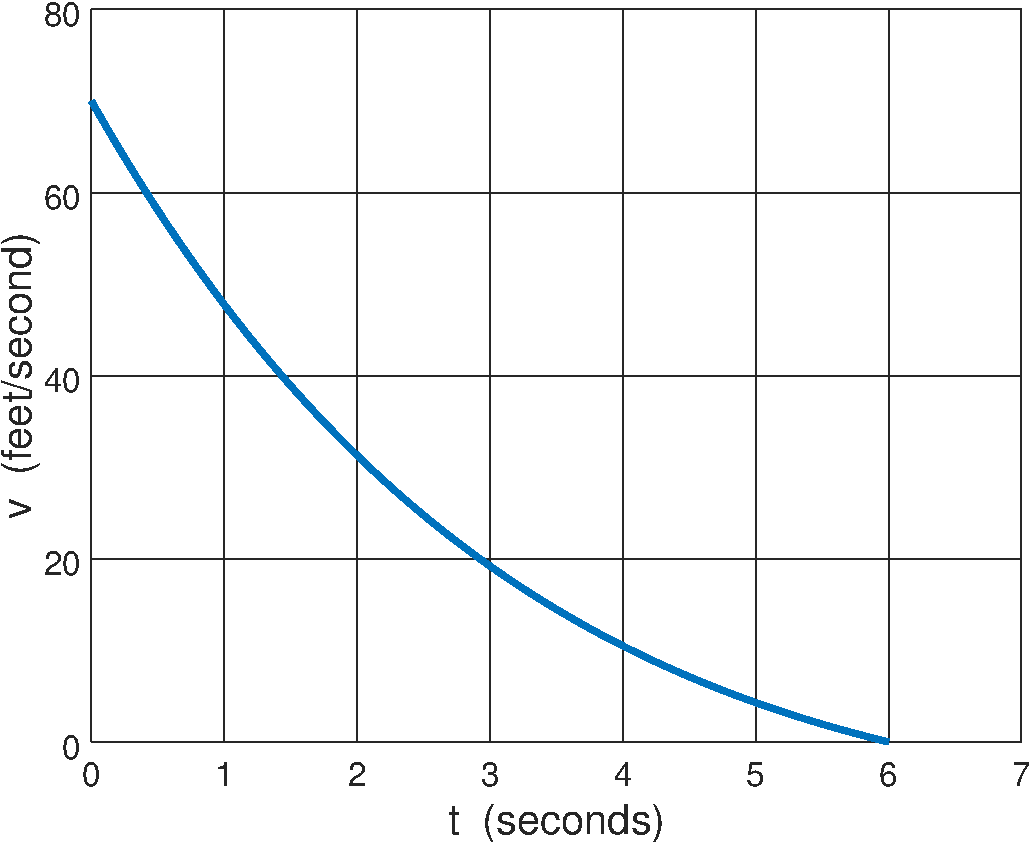
\includegraphics[width=\textwidth]{slowtostop}\end{minipage}
\vspace{1.5in}

\noindent (b) \quad Write the exact distance as a definite integral.
\vspace{1.0in}

% 5.1 #7
\aproblem Evaluate the upper and lower sums for $f(x)=2+\sin x$ on $0 \le x \le \pi$ with $n=4$.  Illustrate with a diagram.
\vfill

\newpage
\thispagestyle{plain}

% 5.2 %39
\aproblem Evaluate the integral by interpreting it in terms of areas.  (\emph{Hint:  Start by sketching the integrand.})
    $$\int_{-4}^3 \left|\tfrac{1}{2} x\right|\,dx \hspace{5.0in}$$
\vfill

% my own
\aproblem  \quad (a)  \quad Set up an expression for the following integral as a limit of sums; you will not be able to compute the limit:
    $$\int_0^5 \arctan x\,dx \hspace{5.0in}$$
\vfill

\noindent (b) \quad Using a graph of $y=\arctan x$, sketch a diagram which shows that
    $$\frac{5\pi}{4} \le \int_0^5 \arctan x\,dx \le \frac{5\pi}{2} \hspace{4.0in}$$
\vfill

\end{aproblems}

\end{document}
